%---
\subsection{Argon Procurement and Purification}
\label{sec:Argon}

A broad strategy has been developed to increase the production of \UAr\ to procure the target required for \DSk.  The \Urania\ project will extract and purify the \UAr\ from the \ce{CO2} wells at the Kinder Morgan Doe Canyon Facility located in Cortez, CO, at a maximum production rate of \UraniaUArRate.  It will be necessary to make a final chemical purification of the \UAr\ before deployment into the \LArTPC\ (driven by the filtration capacity of the getter purification unit), bringing the chemical impurity levels to those shown in Table~\ref{tab:getter}.  Additionally, it would be beneficial to further deplete the \UAr\ of \ce{^39Ar}, giving extended sensitivity to \DSk\ and producing argon with a level of \ce{^39Ar} that is acceptable to be used in an experiment such as \Argo.  The \Aria\ project will serve to chemically purify the \UAr\ to better than the levels shown in Table~\ref{tab:getter} using a cryogenic distillation column called \SeruciOne. The ultimate goal of the \Aria\ project is to process argon through \SeruciOne\ to achieve an additional depletion factor between \AriaDepletionPerPass\ and \AriaDepletionPerTwoPass\ (on top of the reduction of \ce{^39Ar} already seen in the \UAr).  

The procurement of the \UAr\ for \DSk\ is broken into two main operations, extraction of the \UAr\ by \Urania\ and then chemical purification by \Aria\ using \SeruciOne.  

\begin{table}[t!]
%\rowcolors{3}{gray!35}{}
%\small
\centering
\begin{tabular}{cc}
\hline\hline
\multirow{2}{*}{Element}
			&Inlet Purity\\
			&[\si{ppm}]\\
\hline
\ce{CH_4}	&\SI{<0.25}{}\\
\ce{CO}		&\SI{<0.1}{}\\
\ce{CO_2}	&\SI{<0.1}{}\\
\ce{H_2}	&\SI{<1}{}\\
\ce{H_2O}	&\SI{<1}{}\\
\ce{N_2}	&\SI{<1}{}\\
\ce{O_2}	&\SI{<1}{}\\
\hline
\end{tabular}
\caption[Inlet argon purity required for operation of the \DSk\ getter]{Inlet argon purity required for operation of the \DSk\ getter.}
\label{tab:getter}
\end{table}


%---
\subsubsection{\Urania}
The Urania project will extract at least \UraniaTotalDSkProduction\ of low-radioactivity \UAr, providing the required \DSkTotalMass\ of \UAr\ to fill \DSk.   The \Urania\ project will also lay the groundwork for \UAr\ procurement for future, larger argon-based detectors such as \Argo.  The goal of the \Urania\ project is to build a plant capable of extracting and purifying \UAr\ at a maximum rate of \UraniaUArRate, from the same source of \UAr\ that was used for the \DSf\ detector.  

The opportunity to build \Urania\ has grown from the strong relationship between the \DS\ Collaboration and the Kinder Morgan Corporation. Based on gas analysis of the Cortez stream provided to Kinder Morgan by the \DS\ Collaboration during the extraction of the \DSf\ \UAr\ target, a major industrial partnership between Kinder Morgan and Air Products was established in order to extract helium from the \ce{CO2} at Kinder Morgan's Doe Canyon facility.  The Air Products helium plant began operation in \UraniaHeStartDate\ and presently supplies \UraniaHeNationalReserveFractionEquivalentRate\ of the production rate to the National Helium Reserve. 

The \DS\ Collaboration reached an agreement with Kinder Morgan to feed the \Urania\ plant with a small fraction ($\sim$\UraniaGasFeedFraction) of the gas stream returned to Kinder Morgan by Air Products after helium extraction.  This gas stream holds two significant advantages over the gas stream used to extract the \UAr\ for \DSf: it is completely dehydrated,  and it contains only trace amounts of helium. These features greatly simplify the process for \UAr\ extraction by the \Urania\ plant, while ensuring the same radioactivity levels, or better.  Argon from the active \ce{CO2} wells in southwestern Colorado have been found to contain very low levels of the radioactive isotope  \ce{^39Ar}, with the concentration shown to be a factor of \DSfUArArThreeNineDepletion\ below that of argon derived from the atmosphere \cite{Agnes:2016fz}. In an effort lasting more than \SI{5}{\years}, \DSf\ collaborators at Princeton and Fermi National Accelerator Laboratory (Fermilab) extracted and purified \DSfUArMassDelivered\ of \UAr, slightly more than the  \DSfTotalMass\ needed for the target material in the \DSf\ detector. 

The \Urania\ feed gas stream is \UraniaCOTwoFeedFraction\ \ce{CO2}, plus a few percent of \ce{N2}, one percent \ce{CH4}, \UraniaArFeedFraction\ of \UAr, and traces of higher hydrocarbons.  The processing scheme of the \UAr\ extraction plant is optimized for this feed composition in order to achieve an \UAr\ purity of better than \SI{99.9}{\percent}.  A modular plant consisting of skid-mounted units deployable on concrete platforms is being designed to carry out the processing.

The \UAr\ extraction plant will consist of three gas-processing units, as shown in Fig.~\ref{fig:Urania-PID}, followed by a cryogenic distillation unit.  The gas-processing units are two \ce{CO2} liquefier/strippers followed by a pressure swing adsorption unit (\PSA).   The first liquefier accepts gas at \UraniaGasFeedAvePressure, with a flow rate of \UraniaGasFeedFlow\ and a temperature of \SI{5}{\celsius}.  At these conditions, the \ce{CO2} partially condenses and the stream is separated into 2-phases (gas/liquid) as it goes to the first stripper.  In the column a controlled quantity of heat is given by a hot fluid working between the chiller condenser and the column reboilers.  The light products are vaporized and recovered from the top of the column in gas phase.  The heavy products (mainly \ce{CO2}) are collected from the bottom, compressed to \UraniaGasReturnPressure\ and returned to Kinder Morgan as a liquid. The light products coming from the column head are cooled down in the second step to approximately \SI{-50}{\celsius} and sent to the second stripper.  The first column produces \UraniaFirstUnitOutputFlow\ of product flow, a factor of \UraniaFirstUnitFlowReduction\ reduction in the amount of gas to be processed by the more complex downstream units.  

\begin{figure*}[!t]
\centering
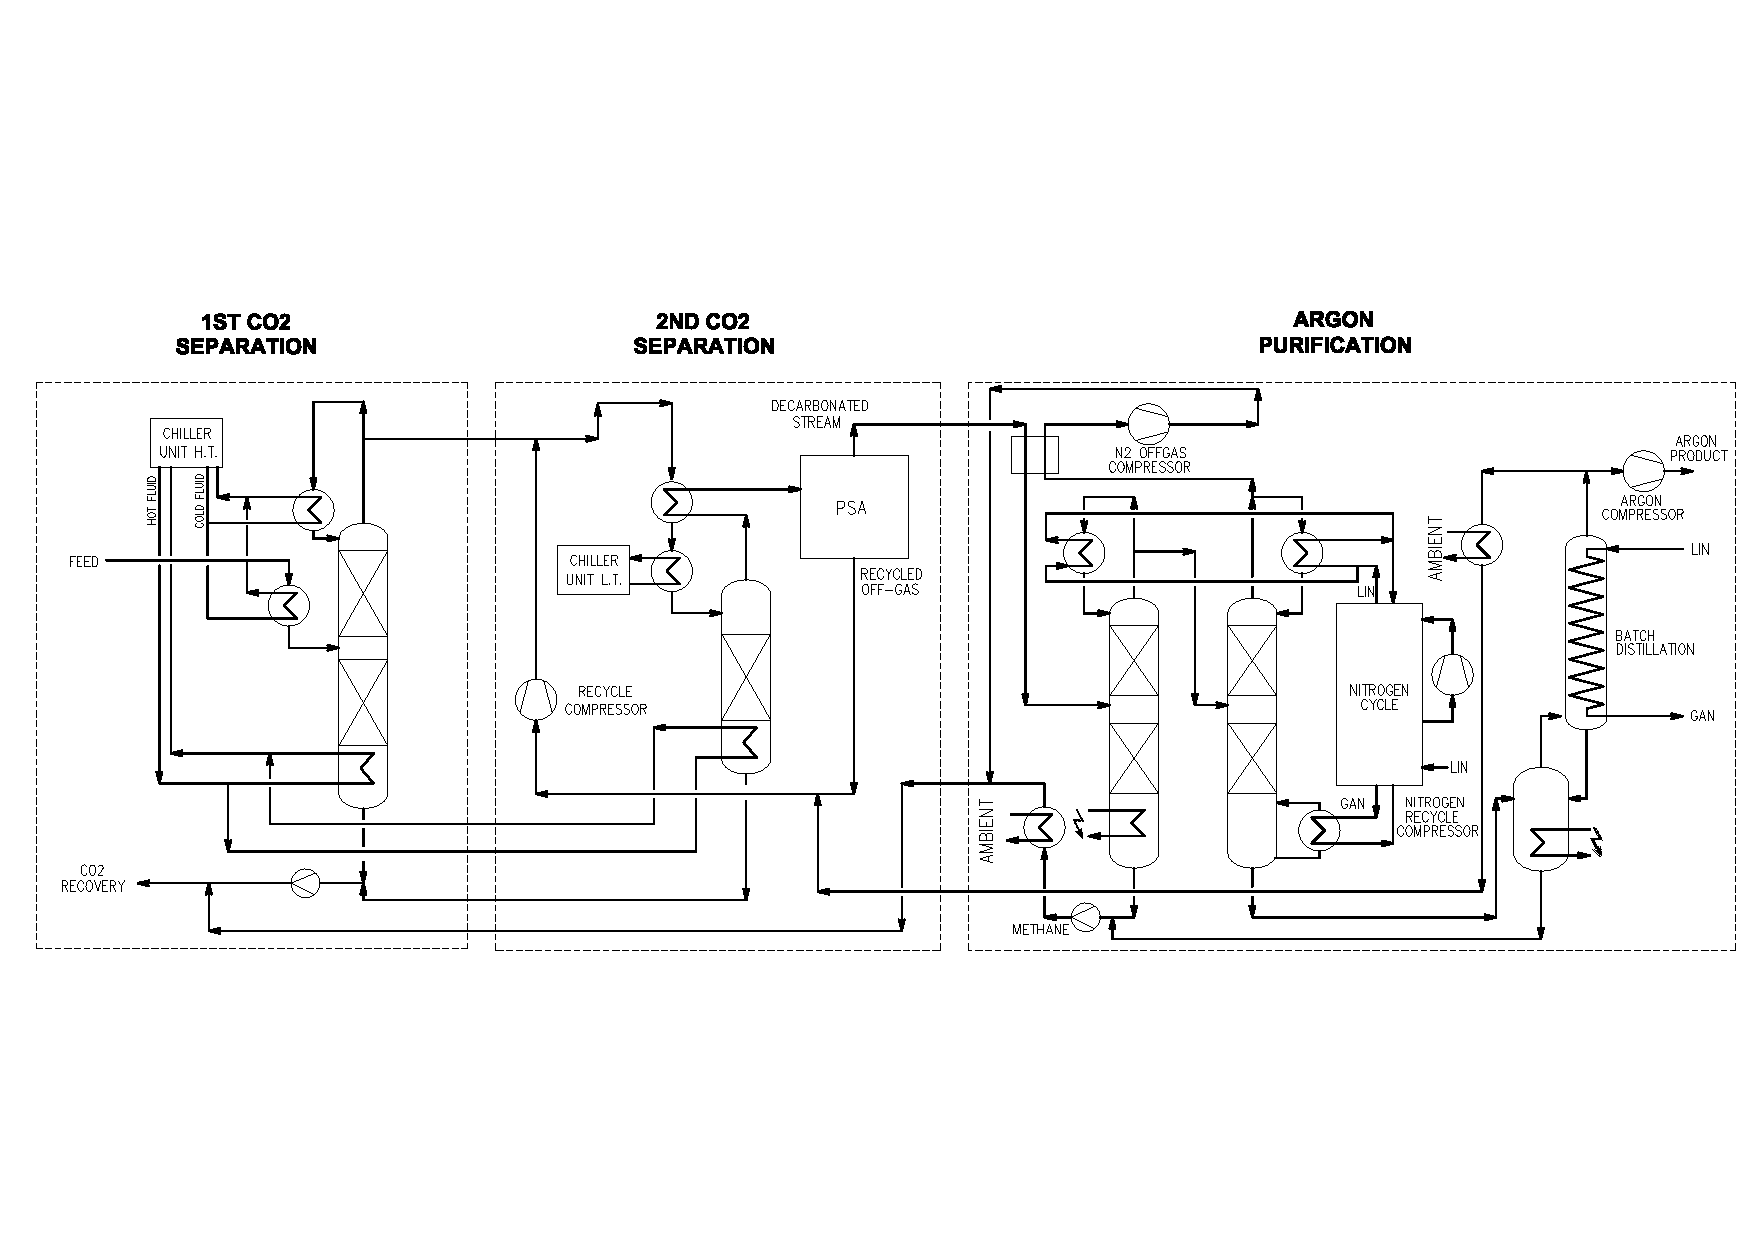
\includegraphics[rotate=90, height=\textheight]{./Figures/Urania-PID.pdf}
\caption[Process Flow Diagram for the \Urania\ \UAr\ extraction plant]{Process Flow Diagram (PFD) for the \Urania\ \UAr\ extraction plant.}
\label{fig:Urania-PID}
\end{figure*}

The second liquefaction and stripping unit further reduces the \ce{CO2} content, in a similar process as the first stripping unit. The separated \ce{CO2} is joined with that from the first unit and returned to Kinder Morgan.  The product gas from the second stripper is re-heated in a heat exchanger and delivered to the \PSA\ unit, which separates the light fractions, including the argon, from the remaining \ce{CO2}.   The \PSA\ is composed of four adsorption beds to allow continuous operation with short time adsorption cycles.  The desorption of \ce{CO2} is made by decreasing the pressure on the bed.  To optimize the performances, the operation of the adsorbers are combined by coupling the purge and pressure swing phases.  At the outlet of the \PSA\ adsorption tanks, one buffer tank is provided in order to dampen process fluctuations and allow for continuous operations of the final distillation process.  The \PSA\ off-gas is delivered to a recycle compressor and sent back to the second \ce{CO2} stripper inlet for reprocessing.  

The \PSA\ is the most critical unit of the entire process since the dynamic adsorption conditions are the most difficult to simulate and predict.  Optimization of the sorbent and other operational parameters is being done via a small scale lab setup in which breakthrough tests are being performed for a variety of gas species. A screening test setup for the \Urania PSA sorbent, is in use at Universit\`a degli Studi di Napoli ``Federico II'' for the characterization and selection of sorbents for the PSA unit of \Urania. Sorbent screening relies on measurements of the breakthrough curves of the different gas species for the candidate sorbents.  A selection of sorbents which could work for the \PSA\ unit have already been identified, while the final selection of the exact sorbent to be used in the \UAr\ extraction plant will be determined by the test results and consultation with the contracted company who will build the plant.

%\begin{figure}[!t]
%\centering
%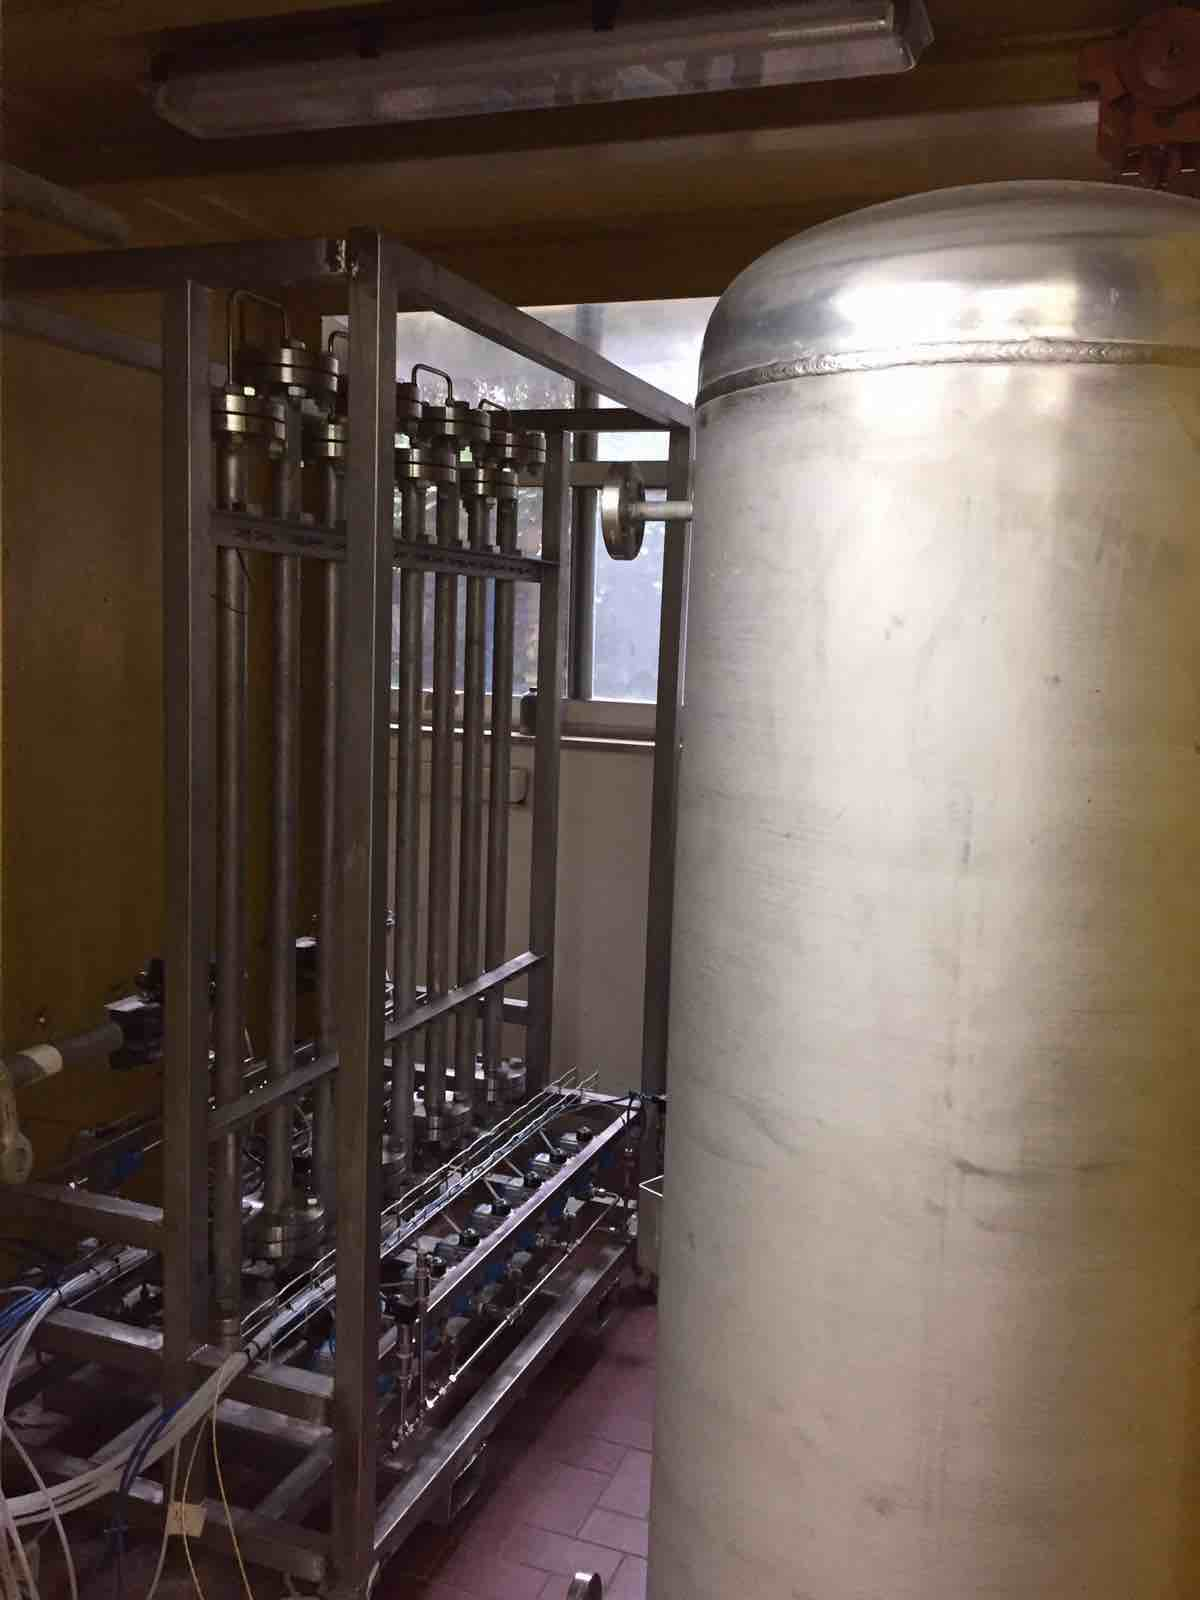
\includegraphics[width=0.45\textwidth]{./Figures/Urania-PSATestPlant.jpg}
%\caption[Screening test plant for the \Urania\ PSA sorbent]{Test plant in use at Universit\`a degli %Studi di Napoli ``Federico II'' for the characterization and selection of sorbents for the PSA unit %of \Urania.}
%\label{fig:Urania-PSATestPlant}
%\end{figure}

The final unit of the \UAr\ extraction plant consists of three cryogenic distillation columns.  The \ce{CO2}-free product coming from the \PSA\ plant is pre-cooled and sent to the first column, which works at a lower pressure (\SI{\sim9}{\barg}) for the removal of \ce{CH4}.  The second column is used to remove the remaining light fractions from the resulting \ce{N2}-rich stream, and the third to perform the final purification of the \UAr\ using a batch distillation process.  In addition to removing the \ce{CH4} and \ce{N2} at this point, any \ce{^85Kr} present in the stream will also be removed by the series of three cryogenic distillation columns.  The \ce{CH4}-rich and \ce{N2}-rich distillation wastes are returned to Kinder Morgan along with the \ce{CO2}.  The final product, \UraniaArFinalPurity\ pure \UAr, will be taken in liquid form from the top of the last column and a small portion collected into a tank to check the quality of the argon.  The majority of the liquid \UAr\ will be sent to the appropriate cryogenic vessels for shipment to Sardinia, where it will undergo final chemical purification by the \SeruciOne\ column.

The Urania project has recently made significant strides, most importantly with the closing of the tender for the construction and shipment of the argon extraction plant by the \INFN\ and announcement of the winner.  The closing of the tender has been done withing the proposed schedule, and the timeline for the extraction of the \UraniaTotalDSkProduction\ of \UAr\ required for the \DSks\ experiment has now been set and integrated with the overall project schedule.  It is now expected that the execution of the contract for the production of the plant will be done in the fourth quarter of the 2019 calendar year.  

The plant will be delivered to the Kinder Morgan Doe Canyon Facility in the first month of 2021. The current plan is to install and commission the plant in the first three quarters of the 2021 calendar year, allowing for extraction of the \UraniaTotalDSkProduction\ of \UAr\ by the middle of the 2022 calendar year, in order to meet the \DSk\ schedule. The preparation of the extraction site is being planned now and will be managed by the collaboration with help from the Kinder Morgan CO2 Company and the contractors hired to carry out the work. Site preparations for developing the facility before the arrival and installation of the plant will begin as soon as the necessary land development permits have been secured and the RFQ process has been completed. 

%The shipment from Colorado to Sardinia will be done by boat in order to minimize the cosmic activation of the argon. For the shipment of the \UAr\ from Colorado, two options are under investigation.   The first option, which was determined to be the baseline method, is to ship the \UAr\ in liquid phase using custom built cryogenic vessels.  This is a more efficient and cost effective method, compared to shipping the \UAr\ in gas phase. The custom built cryogenic vessels will have a double wall structure, there will be two inner volumes with the larger one containing the \UAr\ and the smaller containing \LIN.  The outer volume would be at ultra-high vacuum to thermally insulate the two inner volumes from the atmosphere at ambient temperature.  During the transport, a \LIN\ fed condenser would slowly re-liquify the \UAr\ as it evaporated away, ensuring that none of the \UAr\ would be lost during the trip.  
%A schematic view of the cryogenic vessel design is shown in Fig.~\ref{fig:Urania-UArShipping}.  
%A minimum of five cryogenic vessels is foreseen enabling one for \Urania\ production, one for \Aria\ feed, one for \Aria\ production, and two traveling between Sardinia and LNGS for delivery and then LNGS and Sardinia for further production of \UAr, at all times.

%\begin{figure}[!t]
%\centering
%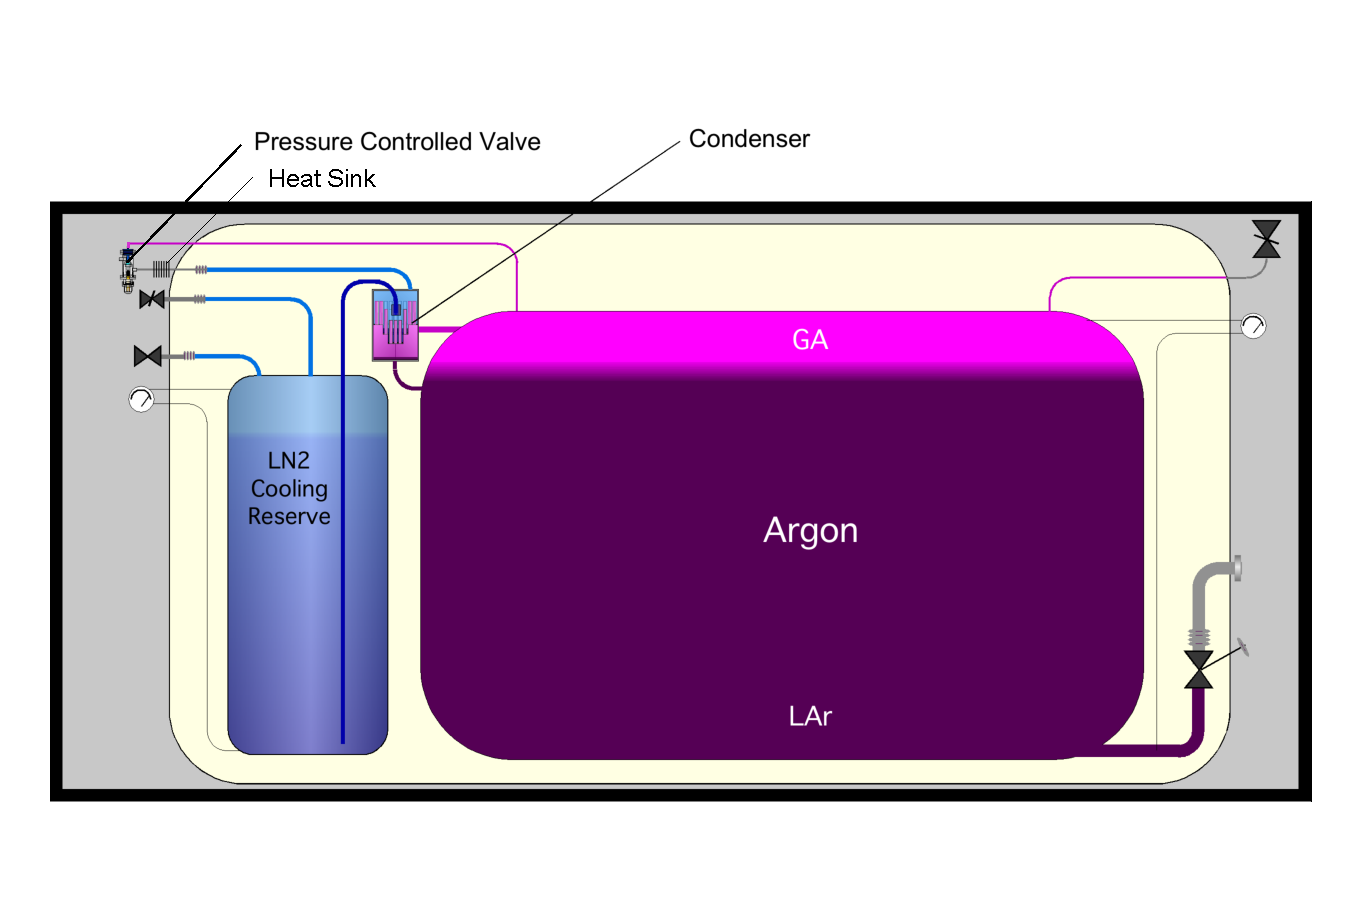
\includegraphics[width=\textwidth]{./Figures/Urania-UArShipping.pdf}
%\caption[Schematic view of \UAr\ cryogenic shipping %vessel]{Schematic view of the cryogenic shipping vessel design, one of the two options for argon shipment from Colorado to Sardinia.}
%\label{fig:Urania-UArShipping}
%\end{figure}

%In the case of cryogenic shipping, the extracted \UAr\ will be shipped to Sardinia in batches of \UraniaUArShipmentMass\ (roughly every \SI{100}{\days}) in liquid phase, also eliminating the need to liquify the \UAr\ to be reprocessed by the \Aria\ column. After chemical purification in \Aria, the \UAr\ will then be shipped to \LNGS, also in batches of \UraniaUArShipmentMass, and stored in the argon recovery system.  In order to minimize the exposure to cosmic rays, the argon will be stored underground at Seruci and/or \LNGS\ for any necessary long durations.

The shipment from Colorado to Sardinia will be done by boat in order to minimize the cosmic activation of the argon. For the shipment of the \UAr\ from Colorado, the current baseline design is to ship the \UAr\ in high-pressure gas cylinders placed in trailer skids which can be hauled by trucks.  This option is made possible by special cylinders which allow for the storage of argon at pressures up to \SI{400}{\bar}.  With pressures of this magnitude, and cylinders that are able to be the size of large trailers, the number of trailers that would be required for the total \DSks\ detector target is something that is manageable, on the order of \numrange{10}{20} depending on the storage pressure.  The overall benefit of this option, instead of going with a cryogenic vessel option, is that the gas can be maintained in the cylinders for years without the need of any type of consumable to prevent the loss of the argon.  This would basically eliminate the risk of losing any of the \UAr\ during the transport and storage, other than potential loss of the shipment.  The Urania project team is now collecting all of the information that is required to make the technical and economic assessment of the high-pressure gas cylinder shipping option which will be a commercially available solution.


%---
\subsubsection{\Aria}
The aim of  \Aria\ is to perform chemical purification of the \UAr\ extracted by \Urania.  \Aria\ will also be the test bench to develop active depletion of \ce{^39Ar} from the \UAr\ to possibly provide \DAr\ targets for future larger-scale \LAr\ detectors.  \Aria\ consists of a \AriaSeruciHeight\ tall distillation column, \SeruciOne, capable of separating isotopes with cryogenic distillation, a process that exploits the tiny difference in volatility due to the difference in isotopic mass~\cite{Lindemann:1919bq,Urey:1932gl,deBoer:1948br,deBoer:1948fc,deBoer:1939cs,Bigeleisen:1961cm}.

The design of the plant started in April~2015 with seed funding from the US NSF through \grant{PHY}{1314507}.  \Aria\ is to be installed in a underground  vertical shaft of  \AriaMonteSinniDiameter\ diameter and \AriaSeruciHeight\ depth,  located at the Seruci mine campus of CarboSulcis, a mining company owned by the Regione Autonoma della Sardegna (\RAS).  In February~2015 a proposal was submitted to the Italian \INFN\ and \RAS, and the funding for the \SeruciOne\ column was approved on July 24, 2015.  Construction of \SeruciOne\ modules started in September 2015 in a Italian company.    

The measurements of the relative volatility of argon isotopes~\cite{Boato:1962hg,Boato:1961hb,Boato:1959bn} and their theoretical interpretation~\cite{Casanova:1964gm,Casanova:1960dj,Fieschi:1961cd} marked the birth of the Italian school of condensed matter in Genoa and Milan.  The study of the relative volatility of argon isotopes was recently revisited~\cite{CanongiaLopes:2003ju,Calado:2000iq} and shows a promising path for the separation of \ce{^39Ar} from \ce{^40Ar}.  Following these studies, \DS\ collaborators developed the framework for comparing \ce{^39Ar} to \ce{^40Ar}.  Algorithms developed to calculate the relative volatility of argon isotopes, based on the extensive and detailed models available in the literature, predict that the volatility of \ce{^39Ar} relative to \ce{^40Ar} is \AriaArVolatiityRatio, and that it stays constant within theoretical uncertainties in the range of temperatures practical for the distillation of argon (\AriaArDistillationTemperatureRange).  The small volatility difference can be used to achieve active isotopic separation by using a cryogenic distillation system with thousands of equilibrium stages.

The design of the \Aria\ plant was optimized on the basis of high-precision numerical methods for estimating the isotopic separation of \ce{^39Ar} from \ce{^40Ar}.  \DS\ Collaborators developed two independent numerical codes, one based on the McCabe-Thiele method~\cite{McCabe:1925be}, and a second based on the Fenske-Underwood-Gilliland (FUG) method and its derivative, the Wynn-Underwood-Gilliland (WUG) method~\cite{Underwood:1949dw,Gilliland:1940ja,Fenske:1932do}.  Calculations for the isotopic separation power of \ce{^39Ar} from \ce{^40Ar} and of the processing rate were performed with the custom codes, as well as with software routines supported by commercial chemical engineering CAD programs, such as Aspen~\cite{AspenTechnologyInc:2015ux}.

Fig.~\ref{fig:Aria-Block-Diagram} illustrates the core of the process for isotopically separating \ce{^39Ar} from \ce{^40Ar}. The process consists mainly of two loops: the process loop where the argon is distilled and the \ce{^39Ar} is separated from the \ce{^40Ar}, and the refrigeration loop where nitrogen gas and liquid is used to evaporate and to condense the argon. Most of the heat is recovered, thanks to the compressor that pumps the nitrogen gas evaporated in the condenser to the reboiler and to the pumps that move the liquid nitrogen produced in the reboiler to the condenser, making the system as efficient as possible.  In Fig.~\ref{fig:Aria-Block-Diagram} all the sub-parts of the plant are represented:
\begin{compactitem}
\item Feed station, to filter and regulate the feed to the column;
\item Compressor station, to bottle the distillate at the bottom;
\item Vacuum system, to keep a good vacuum in the cold-box, in order to minimize the heat losses;
\item \ce{LN2} storage;
\item Nitrogen condenser system, consisting of 4 Stirling cryo-refrigerators needed to re-condense the nitrogen, used in a closed loop.
\end{compactitem}

\SeruciOne\ will consist of \AriaCentralModulesNumber\ modules of \AriaCentralModulesHeight\ height, plus a top module (condenser) and a bottom module (reboiler). 
% \SeruciOne\ will serve to prove the isotopic separation power of the cryogenic distillation method.  \SeruciOne.  All modules will be pre-assembled at the factory and ready for deployment in the shaft.  The refurbishment of the \SeruciOne\ mine shaft is now well underway, in order to make it suitable to host the column.  The availability of the unused well in the mining site of \SeruciOne\ to house the column will allow for the construction of the plant with minimal environmental impact and relatively low cost. Once completed, it will be the highest distillation column in the world. 

\begin{figure*}[!t]
\centering
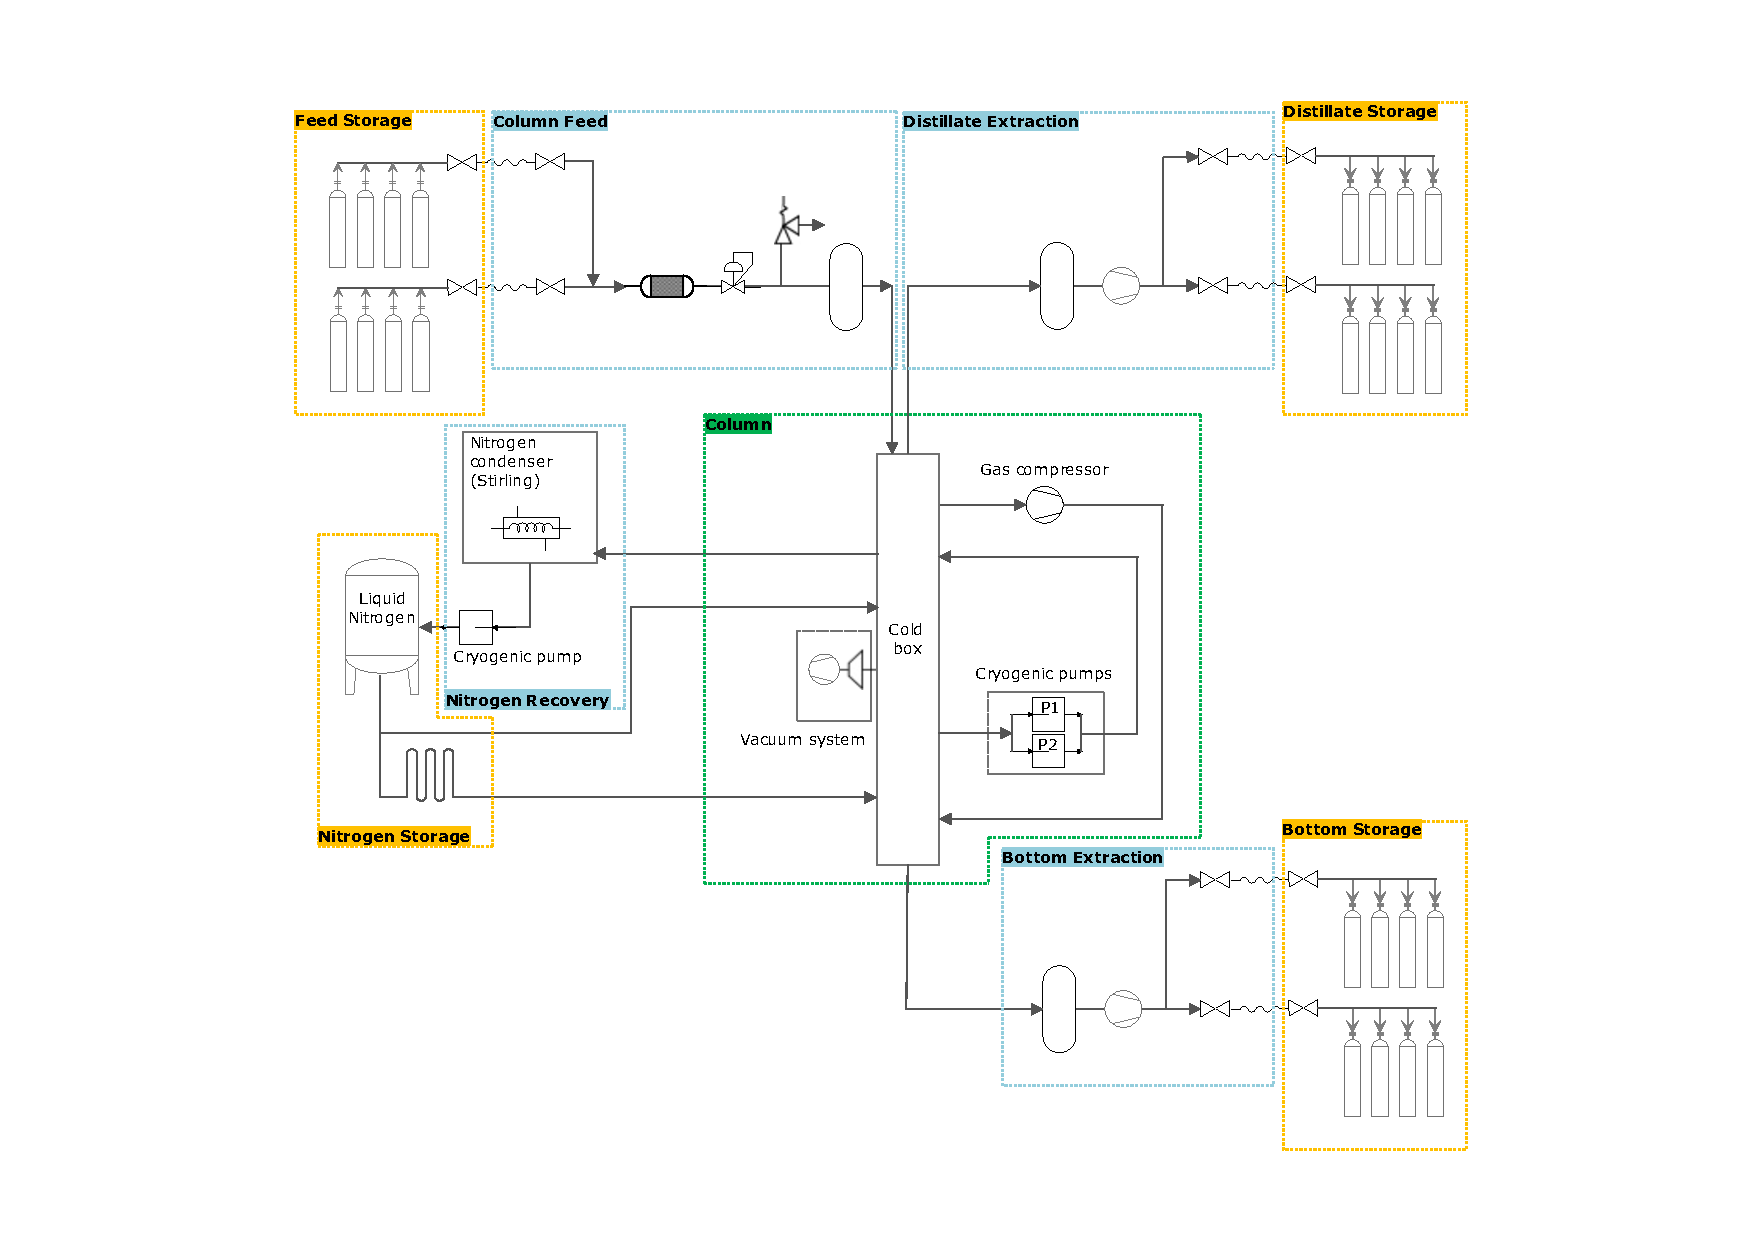
\includegraphics[width=\textwidth]{./Figures/Aria-Block-Diagram.pdf}
\caption[Block diagram of \Aria]{Block diagram of the cryogenic system of the \Aria\ plant.}
\label{fig:Aria-Block-Diagram}
\end{figure*}

Calculations indicate that \SeruciOne\ will be able to process \UAr\ at a rate of \AriaChemicalRate\ removing all chemical impurities (including traces of \ce{N2}, \ce{O2}, and \ce{Kr}) with a separation power better than \AriaChemicalPerPass\ per pass.  Additionally, \SeruciOne\ can be used in a different mode of operations to test the isotopic separation of the argon, in order to further reduce the \ce{^39Ar} content in the \UAr.  The same models which have been used to calculate the chemical purification rate, have also been used to show that \SeruciOne\ would be able to isotopically separate the \UAr\ at a rate of \AriaSeruciOneRate, while obtaining an \ce{^39Ar} depletion factor of \AriaDepletionPerPass\ per pass. 

All modules for \SeruciOne\ have already been built and passed a series of quality assurance checks.  During the first check, the process column and all the service pipes were individually checked for leaks at room temperature.  Then, the pipes were wrapped with super-insulation and everything was assembled into the cold box.  The second check was a full module check, with an additional check done on the bottom reboiler module at \SI{77}{\kelvin}.  To date, all modules have passed both checks at room temperature and the bottom module has passed the final cold temperature check.  

\SeruciZero\ is a  test column,  installed in a outdoor assembly hall at Nuraxi Figus, Italy, seen in Figure~\ref{fig:SeruciZero}, that is made with the  \SeruciOne\ top and bottom modules and  a single central module.  The goal  of \SeruciZero\ is  to confirm the proper operation of the three main components of the \SeruciOne\ column, as well as to gain experience in operating the column on a smaller scale and to put in place the standard operating procedures.  
During the month of July 2019 the test column was put in operation with nitrogen both as refrigerant and liquid to be distilled. Stable distillation conditions were reached during more than two weeks time. A new run is foreseen during October 2019 to precisely determine distillation parameters and verify the theoretical predictions. A run with argon is also foreseen to test the plant operation with the final gas.

\begin{figure*}[!t]
\centering
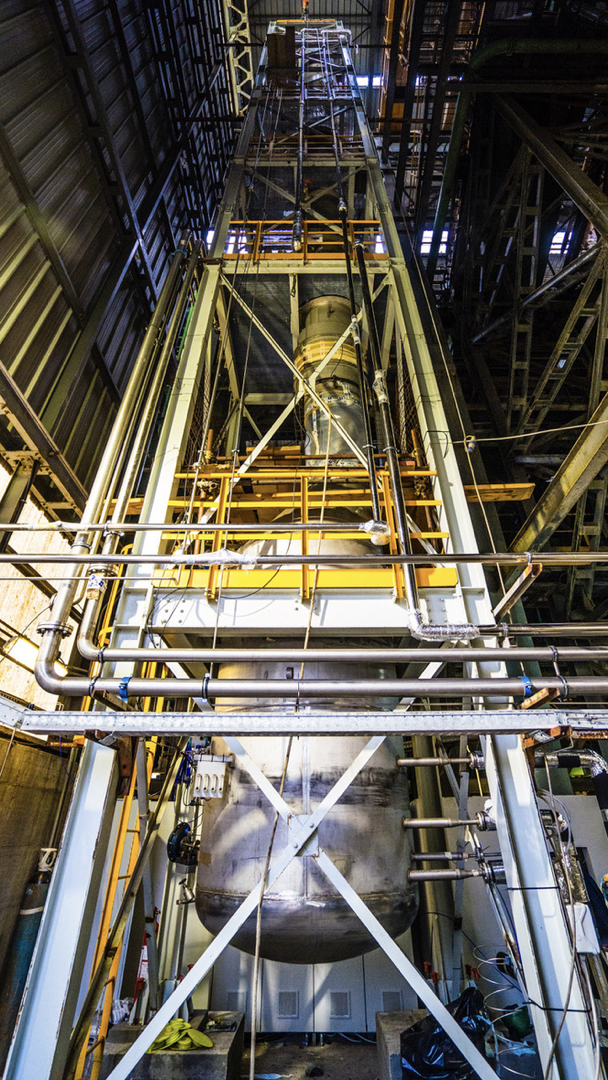
\includegraphics[height=0.95\textheight]{./Figures/Aria.png}
\caption[The \SeruciZero\ cryogenic distillation column]{The \SeruciZero\ cryogenic distillation column, installed in the {\it Laveria} building of Carbosulcis in Nuraxi Figus, Sardinia, Italy.}
\label{fig:SeruciZero}
\end{figure*}

% old text in NSF IDR
%Concerning the installation of \SeruciOne, all the documents needed for the authorization request for installation were submitted in May 2018 to the competent authorities. During the first half of 2019, several meetings have been held, both with the fire brigade and with other local and county offices, entities and authorities. The authorization were eventually obtained.  During  2018 a complete cleaning and preparation of the well at the Seruci site has been performed.  A well-defined coring procedure was concluded in 2018. After the examination of the rocks samples, the design for the \SeruciOne\ supporting structure was detailed. The tender was completed in Autumn 2018, and at the beginning of 2019 a carbon steel sample platform was delivered to the mine  and installed in the Seruci well.  The test was successful and was very useful in order to define all  installation steps. 
%The goal is to receive all of the platforms by the end of May 2019 and to install them inside the  well by the end of 2019.

% update text from W.Bonivento (30/9/19)
Concerning the installation of \SeruciOne, all  authorizations were eventually obtained.  During  2018 a complete cleaning and preparation of the well at the Seruci site has been performed.  A well-defined coring procedure was concluded in 2018. After the examination of the rocks samples, the design for the \SeruciOne\ supporting structure was detailed. All the platforms were delivered. Installations of the first platforms in the well has started.


%An additional storehouse has been selected in order to provide a ``confined area'' for storage and for operations at the Seruci site. It has been completely refurbished and equipped with TV-CC system for security monitoring.  To date, 15 of the remaining 27 \SeruciOne\ central modules have been stored in the \SeruciZero\ warehouse, while the other 12 of them are stored in the \SeruciOne\ warehouse. 

\subsubsection{\DArT} 
The \DArT\ experiment will re-use the \ArDM\ infrastructure with minimal modifications made and will consists of a radio-pure single-phase \LAr\ detector with about one liter contained inside of its active volume.  The \DArT\ detector itself will be placed inside the middle of the \ArDM\ vessel.  \DArT\ will be filled with argon to be tested in order to measure the content of \ce{^39Ar}.  The detector will be readout by two cryogenic \SiPMs\ each with a surface area of \DSkSiPMAreaMaxcm.  The \SiPMs\ and the readout electronics will come from the \DSks\ production chain. 

The \ArDM\ detector will act as an active veto against internal and external radiation. For this purpose, we are building a dedicated single phase setup with a new set of low-radioactive photo-multipliers (PMT). However, we will also retain the entire present double phase setup for later use, e.g.~for measurements of large quantities of depleted argon.

Extensive GEANT4-based simulations were performed using the Monte Carlo simulation package inherited from the \DSf.  These simulations show that  \DArT\  will  achieve a sub-\DArTUArPercentErrorWithoutLeadWithDepletionTen\ measurement when operated inside the \ArDM\ detector, for \ce{^39Ar} concentrations a factor of ten smaller that those of \AAr, and in about a week of running.  A \DArTUArPercentErrorWithoutLeadWithDepletionHundred\ measurement could be made for \ce{^39Ar} concentrations as low as two orders of magnitude (statistical uncertainty only) smaller than those in \AAr. This setup will also be useful to characterize the performance of \Aria, which is expected to suppress the \ce{^39Ar} content by a factor of \AriaDepletionPerPass\ per pass.  

A very important addition to the setup described above will consist of adding a \DArTLeadBeltMass\ lead belt about \DArTLeadBeltHeight\ tall around the \ArDM\ vessel, at the mid-height position.  This will suppress the impact of external photons that dominate the background budget and allow for the measurement of even larger \ce{^39Ar} depletion factors, corresponding to that of the \UAr.  If the depletion levels are those already measured in the past (i.e. of \DSfUArDepletion), it will be possible, according to our simulations, to measure them with a \DArTUArPercentErrorWithLead\ uncertainty in about a week of running. Upper limits can be set on depletion factors of order \DArTUArDepletionWithLead\ (statistical uncertainty only), i.e. \UAr\ with one  distillation pass in Aria.

The argon from \Urania\ is expected to be available only after mid-2021. However, it is planned that after the run of \DSfs\ at LNGS, presumably at the end of 2019, its argon will be measured with \DArT\ to cross-check the original measurement taken with \DSfs\ and to test the new setup. This  \DArT\  experiment is expected to become a useful facility within LSC for the years to come, since it will be needed to measure samples of the extracted argon from \Urania\ over time.  An Expression of Interest and a TDR were recently submitted to the LSC Directorate. Detector construction in all collaborating institutions has already started.   